\documentclass[final,hyperref={pdfpagelabels=false}]{beamer}
\usepackage{grffile}
\mode<presentation>{\usetheme{PCFC}}
%\usepackage[ngerman]{babel}        % Deutsch, neue Rechtschreibung
\usepackage[english]{babel}       % English  
\usepackage{csquotes}
\usepackage[utf8]{inputenc}
\usepackage{amsmath,amsthm, amssymb, latexsym}
\boldmath
\usepackage[orientation=portrait,size=a0,scale=1.4,debug]{beamerposter}

\usepackage{array,booktabs,tabularx}
\newcolumntype{Z}{>{\centering\arraybackslash}X} % centered tabularx columns
\newcommand{\pphantom}{\textcolor{white}} % phantom introduces a vertical space in p formatted table columns??!!

\listfiles
\usepackage{graphicx}
\usepackage{multicol}
\usepackage[version=3]{mhchem} % Formula subscripts using \ce{}
\newcommand{\nox}{NO$_x$} % our abbreviation
\usepackage{subfigure}
\usepackage{lipsum}

\usepackage[
backend=biber,
doi=true,
sorting=none,
sortcites=true,
maxbibnames=3,
minbibnames=1,
maxcitenames=2,
mincitenames=1,
citestyle=numeric-comp,
giveninits=true,
isbn=false,
date=year
]{biblatex}
\addbibresource{../sample.bib}

%%%%%%%%%%%%%%%%%%%%%%%%%%%%%%%%%%%%%%%%%%%%%%%%%%%%%%%%%%%%%%%%%%%%%%%
%                              @article
%%%%%%%%%%%%%%%%%%%%%%%%%%%%%%%%%%%%%%%%%%%%%%%%%%%%%%%%%%%%%%%%%%%%%%%
\DeclareBibliographyDriver{article}{%
	\usebibmacro{bibindex}%
	\usebibmacro{begentry}%
	\usebibmacro{author/translator+others}%
	\newunit\newblock%
	\setunit*{\addspace}%
	\usebibmacro{doi+eprint+url}%
	\usebibmacro{finentry}
}

% Make sure that URL is not printed if DOI is available
\renewbibmacro*{doi+eprint+url}{%
	\iftoggle{bbx:doi}
	{\iffieldundef{url}{\printfield{doi}}{\iffieldundef{doi}{}{\printfield{doi}}}}
	{}%
	\newunit\newblock
	\iftoggle{bbx:eprint}
	{\usebibmacro{eprint}}
	{}%
	\newunit\newblock
	\iftoggle{bbx:url}
	{\iffieldundef{doi}{\usebibmacro{url+urldate}}{}}
	{}
}

% New macro for @software to print both URL and DOI
\newbibmacro*{doi+url+software}{%
	\iftoggle{bbx:doi}
	{\printfield{doi}}{}%
	\newunit\newblock
	\iftoggle{bbx:url}
	{\usebibmacro{url+urldate}}{}%
}
%%%%%%%%%%%%%%%%%%%%%%%%%%%%%%%%%%%%%%%%%%%%%%%%%%%%%%%%%%%%%%%%%%%%%%%%%%%%%%%%%%%%%%
%this isn't working exactly as desired, but it has potential:
%https://tex.stackexchange.com/questions/74808/how-to-line-up-blocks-in-columns-with-full-width-blocks-in-beamer-beamerposter
\newenvironment<>{varblock}[2][0.96\textwidth]{%
	\setlength{\textwidth}{#1}
	\begin{actionenv}#3%
		\def\insertblocktitle{#2}%
		\centering
		\par%
		\centering
		\usebeamertemplate{block begin}}
	{\par%
		\usebeamertemplate{block end}%
	\end{actionenv}}
%%%%%%%%%%%%%%%%%%%%%%%%%%%%%%%%%%%%%%%%%%%%%%%%%%%%%%%%%%%%%%%%%%%%%%%%%%%%%%%%%%%%%%
 
\title{\huge Reaction Class-Based {CHON} Combustion Mechanism Development}
\author{\LARGE Mark E. Fuller$^1$, K. Alexander Heufer$^1$}
\date{}
\institute{\Large $^1$Physico-Chemical Fundamentals of Combustion\\RWTH Aachen University}

%%%%%%%%%%%%%%%%%%%%%%%%%%%%%%%%%%%%%%%%%%%%%%%%%%%%%%%%%%%%%%%%%%%%%%%%
\begin{document}
\begin{frame} %whole poster is one frame
	
%%varblock styling (needs improvement)	
%	  \begin{columns}[t,totalwidth=\linewidth]
%		\begin{column}{.48\textwidth}
%			\begin{varblock}{\LARGE Introduction}
%				Blarg!
%			\end{varblock}
%		\end{column}
%		\begin{column}{.48\linewidth}
%			\begin{varblock}{\Large Problems are soluble}
%	           	\begin{enumerate}
%					\item Point 1
%					\item Point 2
%				\end{enumerate}	
%			\end{varblock}
%		\end{column}
%	\end{columns}
%	
%	\begin{columns}
%		\begin{column}{.98\textwidth}
%			\begin{block}{Full-width block}
%				\begin{multicols}{2}
%					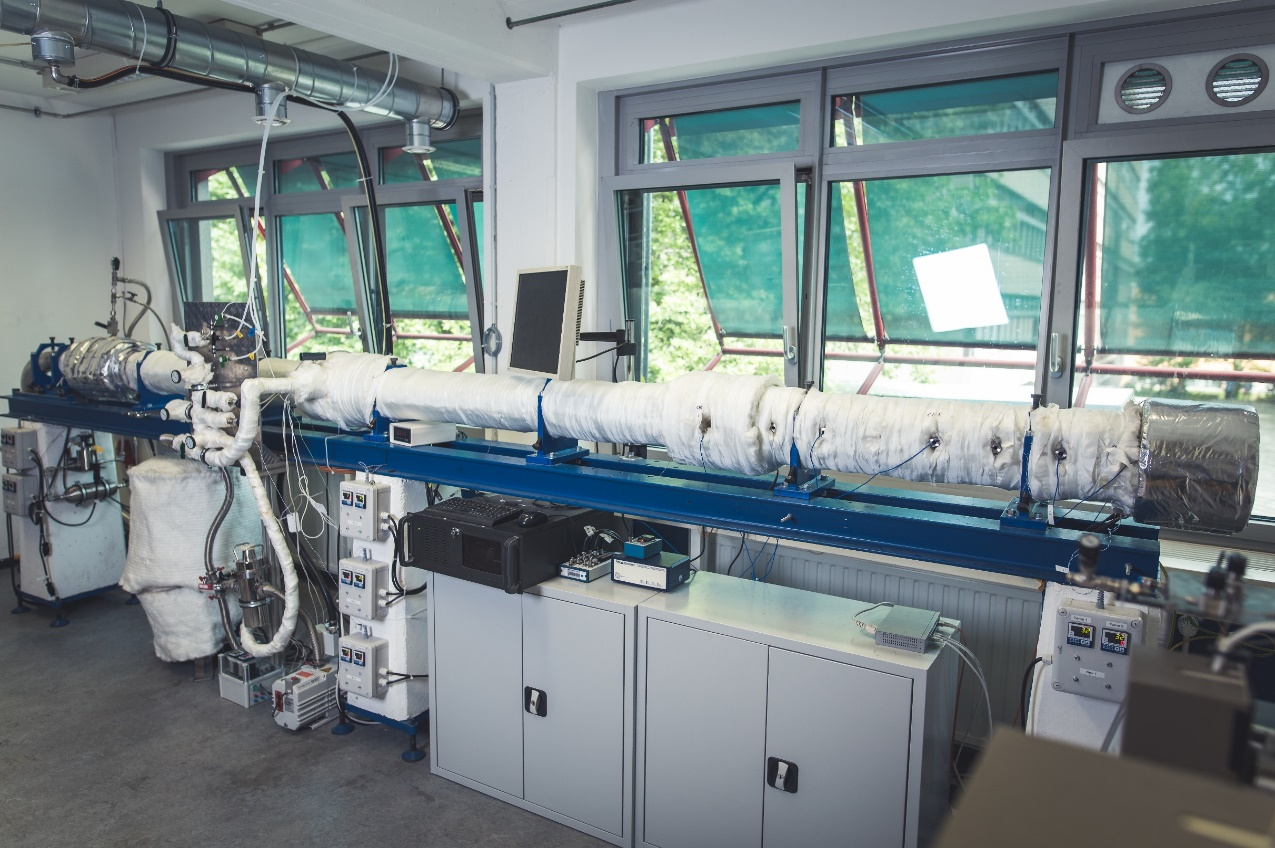
\includegraphics[width=0.9\columnwidth]{../figures/PCFC_ST.jpg}
%					WOW!
%					\columnbreak
%					\begin{enumerate}
%						\item Shock tubes are cool
%						\item Ours is hot!
%					\end{enumerate}	
%				\end{multicols}
%			\end{block}
%		\end{column}
%	\end{columns}
%	
%	\begin{columns}[t,totalwidth=\linewidth]
%		\begin{column}{.5\linewidth}
%			\begin{varblock}{\LARGE Split left}
%				Test citation\cite{Fuller.2014}.
%			\end{varblock}
%		\end{column}
%		\begin{column}{.5\linewidth}
%			\begin{varblock}{\LARGE REFERENCES}
%					\printbibliography
%			\end{varblock}
%		\end{column}
%	\end{columns}	
%\vfill


%old style (more tedious, but ok)
	\begin{columns}
	\begin{column}{.48\textwidth}
		\begin{beamercolorbox}[center,wd=\textwidth]{postercolumn}
			\begin{block}{\LARGE Introduction}
				\begin{itemize}
					\item Interactions of \nox\ (\ce{NO} and \ce{NO2}) with the combustion
process are increasingly relevant in engines with exhaust gas
recirculation (EGR) and/or alkyl nitrate cetane enhancers
					\item Low-temperature combustion reactions with nitrogen are not
well-studied and may have significant effects
					\item Sustainable fuels, produced from bio-based carbon
feedstocks, \ce{CO2} , and renewable electricity, contain additional
functional groups whose reactions with \nox\ are not well-characterized
				\end{itemize}
				\begin{figure}
					\centering
					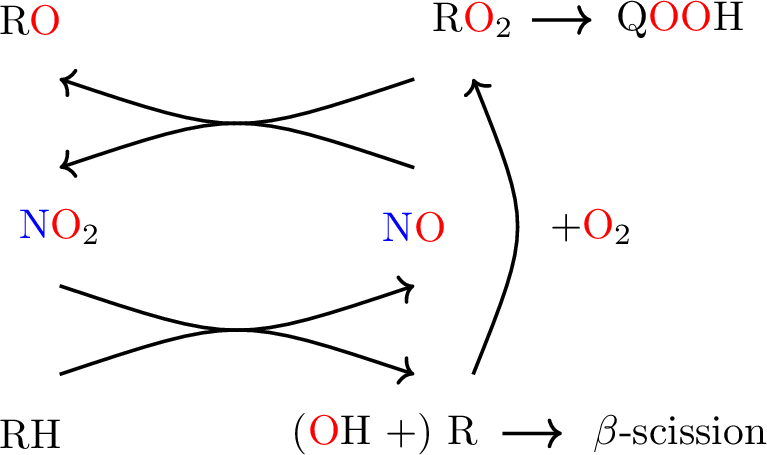
\includegraphics[width=0.7\linewidth]{../figures/NOx_cycle.png}
				\end{figure}
			\end{block}
		\end{beamercolorbox}
	\end{column}
	% end left column
	% ---------------------------------------------------------%
	% start right column
	\begin{column}{.48\textwidth}
		\begin{beamercolorbox}[center,wd=\textwidth]{postercolumn}
			\begin{block}{\LARGE Model Development}
				\begin{itemize}
					\item Pentane isomer mechanism (\ce{CHO}) of Bugler {\it et al.} utilized as \ce{C0}-\ce{C5} base mechanism
				\end{itemize}
				\vspace{5cm}
				\begin{figure}
					\centering
					\includegraphics[width=0.7\linewidth]{../figures/NOx_Cycle.png}
				\end{figure}	
			\end{block}
		\end{beamercolorbox}
	\end{column}
\end{columns}

%fullwidth block
\begin{columns}
	\begin{column}{.98\textwidth}
		\begin{beamercolorbox}[center,wd=\textwidth]{postercolumn}
			\begin{block}{\LARGE Modeling results}
				\begin{multicols}{2}
					\begin{figure}
						\centering
						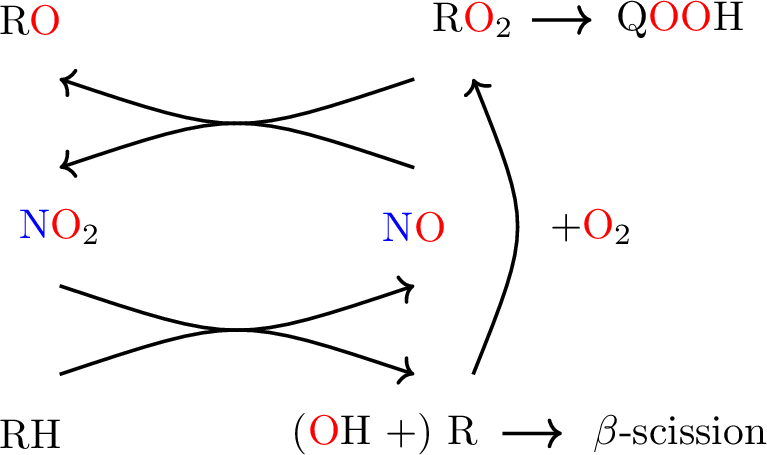
\includegraphics[width=0.8\linewidth]{../figures/NOx_cycle.png}
					\end{figure}
					WOW!
					\columnbreak
					\begin{figure}
						\centering
						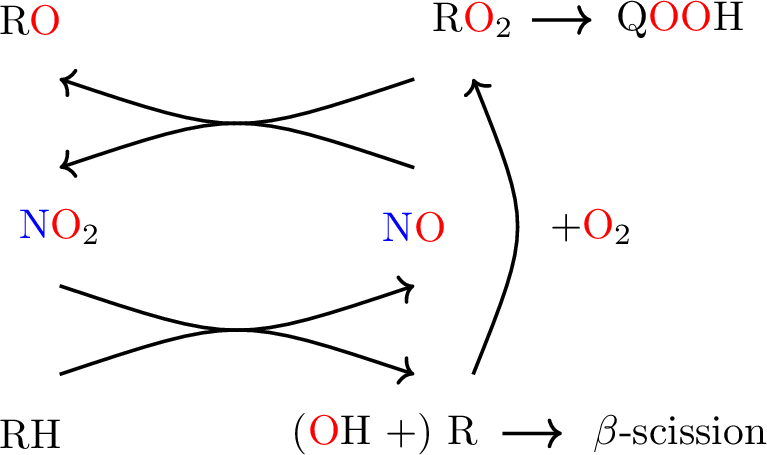
\includegraphics[width=0.8\linewidth]{../figures/NOx_cycle.png}
					\end{figure}
					Check this shit out!
					
				\end{multicols}
			\end{block}
			%\vfill
		\end{beamercolorbox}
	\end{column}
\end{columns}

%back to left /right columns
\begin{columns}
	\begin{column}{.48\textwidth}
		\begin{beamercolorbox}[center,wd=\textwidth]{postercolumn}
			\begin{block}{\LARGE Work-in-progress}
				{\it Ab initio} calculations	
			\end{block}
		\end{beamercolorbox}
	\end{column}
	% end left column
	% ---------------------------------------------------------%
	% start right column
	\begin{column}{.48\textwidth}
		\begin{beamercolorbox}[center,wd=\textwidth]{postercolumn}
			\begin{block}{\LARGE REFERENCES}
				\printbibliography
				
			\end{block}
		\end{beamercolorbox}
	\end{column}
\end{columns}
\vskip2ex



\end{frame}
\end{document}


%%%%%%%%%%%%%%%%%%%%%%%%%%%%%%%%%%%%%%%%%%%%%%%%%%%%%%%%%%%%%%%%%%%%%%%%